\chapter{Proiectarea Hardware \label{hardware_design}}

\begin{figure}[htbp]
    \centering
    \resizebox{0.95\textwidth}{!}{%
    \begin{tikzpicture}[
        >=stealth, thick,
        box/.style={draw=black!70, fill=blue!5, rectangle, rounded corners=2pt, minimum height=0.6cm, text width=2.4cm, align=center, font=\scriptsize\sffamily},
        cots/.style={draw=black!70, fill=orange!10, rectangle, rounded corners=6pt, minimum height=0.6cm, text width=2.4cm, align=center, font=\scriptsize\sffamily},
        pwr/.style={draw=black!70, fill=red!15, rectangle, rounded corners=3pt, minimum height=0.8cm, text width=4cm, align=center, font=\scriptsize\sffamily},
        io/.style={font=\scriptsize\sffamily\bfseries, align=center}
    ]

    % --- Core DSP ---
    \node[cots, minimum height=8.5cm, text width=2cm] (dsp) at (0, 0) {Procesor\\Digital de\\Semnal\\(DSP)};
    
    % --- Programator ---
    \node[cots, above=1cm of dsp] (prog) {Programator DSP};
    \node[io, left=0.8cm of prog] (conn_usb) {Port USB};
    \draw[->] (conn_usb) -- (prog);
    \draw[<->] (prog) -- (dsp) node[midway, right, font=\scriptsize] {I2C};

    % --- Inputs ---
    \node[box] (in_bal1) at (-4, 2.5) {Interfață\\Echilibrată};
    \node[box] (in_bal2) at (-4, 0.0) {Interfață\\Echilibrată};
    \node[box] (in_unbal) at (-4, -2.5) {Interfață\\Neechilibrată};

    \node[io] (conn_in_bal1) at (-6.5, 2.5) {XLR / TRS};
    \node[io] (conn_in_bal2) at (-6.5, 0.0) {XLR / TRS};
    \node[io] (conn_in_unbal) at (-6.5, -2.5) {Jack 1/4"};

    \draw[->] (conn_in_bal1) -- (in_bal1);
    \draw[->] (conn_in_bal2) -- (in_bal2);
    \draw[->] (conn_in_unbal) -- (in_unbal);

    \draw[->] (in_bal1.east) -- (dsp.west |- in_bal1.east);
    \draw[->] (in_bal2.east) -- (dsp.west |- in_bal2.east);
    \draw[->] (in_unbal.east) -- (dsp.west |- in_unbal.east);

    % --- Outputs ---
    \node[box] (out_bal1) at (4, 3.8) {Ieșire\\Echilibrată};
    \node[box] (out_bal2) at (4, 2.7) {Ieșire\\Echilibrată};
    \node[box] (out_bal3) at (4, 1.6) {Ieșire\\Echilibrată};
    \node[box] (out_bal4) at (4, 0.5) {Ieșire\\Echilibrată};

    \node[cots] (out_pwr1) at (4, -0.7) {Amplificator\\Clasa D};
    \node[cots] (out_pwr2) at (4, -1.8) {Amplificator\\Clasa D};
    \node[cots] (out_pwr3) at (4, -2.9) {Amplificator\\Clasa D};
    \node[cots] (out_pwr4) at (4, -4.0) {Amplificator\\Clasa D};

    \foreach \i/\y in {1/3.8, 2/2.7, 3/1.6, 4/0.5} {
        \node[io] (conn_out_bal\i) at (6.5, \y) {XLR / TRS};
        \draw[->] (out_bal\i) -- (conn_out_bal\i);
        \draw[->] (dsp.east |- out_bal\i.west) -- (out_bal\i.west);
    }
    \foreach \i/\y in {1/-0.7, 2/-1.8, 3/-2.9, 4/-4.0} {
        \node[io] (conn_out_pwr\i) at (6.5, \y) {Conectori\\Banană};
        \draw[->] (out_pwr\i) -- (conn_out_pwr\i);
        \draw[->] (dsp.east |- out_pwr\i.west) -- (out_pwr\i.west);
    }

    % --- Power ---
    \node[pwr] (power) at (0, -6.0) {Convertor DC-DC\\+ Masă virtuală};
    
    % 12V IN
    \node[io] (conn_pwr) at (-4, -6.0) {12V DC IN};
    \draw[->] (conn_pwr) -- (power.west);

    % --- Power Routing (Bottom Taps & Trimmed Buses) ---
    % DSP 5V
    \draw[->, dashed, red!80!black, thick] (power.north) -- (dsp.south) node[midway, right, font=\scriptsize] {5V};
    
    % Left Bus - FAR LEFT (X=-8.5)
    \draw[dashed, red!80!black, thick] (power.north west) ++(0,-0.2) -- (-8.5, -5.8) coordinate (bus_L);
    \draw[dashed, red!80!black, thick] (bus_L) -- (-8.5, 2.0) node[pos=0.8, right, font=\scriptsize] {12V + VGND};
    
    % Left Taps - Enter from bottom (South)
    \foreach \y in {2.5, 0.0, -2.5} {
        \draw[->, dashed, red!80!black, thick] (-8.5, \y - 0.6) -- (-4, \y - 0.6) -- (-4, \y - 0.3);
    }

    % Right Bus - FAR RIGHT (X=8.5)
    \draw[dashed, red!80!black, thick] (power.north east) ++(0,-0.2) -- (8.5, -5.8) coordinate (bus_R);
    \draw[dashed, red!80!black, thick] (bus_R) -- (8.5, 3.3);
    
    \node[left, text=red!80!black, font=\scriptsize, fill=white, inner sep=1pt] at (8.4, 0.2) {12V + VGND};
    \node[left, text=red!80!black, font=\scriptsize] at (8.4, -2.0) {12V};

    % Right Taps - Enter from bottom (South)
    \foreach \y in {3.8, 2.7, 1.6, 0.5} {
        \draw[->, dashed, red!80!black, thick] (8.5, \y - 0.6) -- (4, \y - 0.6) -- (4, \y - 0.3);
    }
    \foreach \y in {-0.7, -1.8, -2.9, -4.0} {
        \draw[->, dashed, red!80!black, thick] (8.5, \y - 0.6) -- (4, \y - 0.6) -- (4, \y - 0.3);
    }

    \end{tikzpicture}
    }
    \caption{Diagrama bloc funcțională a sistemului.}
    \label{fig:block_diagram_sys}
\end{figure}

Acest capitol detaliază arhitectura hardware a amplificatorului audio multicanal, ilustrând metodologia de proiectare, selecția componentelor și integrarea acestora la nivel de sistem. Concret, capitolul va descrie dezvoltarea etajelor electronice proiectate: interfețele audio de linie pentru intrare și ieșire și sistemul de alimentare cu masă virtuală. 

Pentru a eficientiza dezvoltarea, anumite funcții complexe au fost implementate utilizând module pre-asamblate. Astfel, designul a trebuit să acomodeze și să interconecteze corect procesorul digital de semnal, amplificatoarele de putere în clasa D și programatorul hardware al DSP-ului. Designul rezultat este prezentat în Figura \ref{fig:block_diagram_sys}.

\section{Sistemul de alimentare și masa virtuală}
Alimentarea circuitelor analogice se realizează de la o sursă unipolară de $12\text{ V}$. Deoarece semnalele audio sunt în esență bipolare (oscilează în jurul unei referințe de $0\text{ V}$), utilizarea unei singure surse de alimentare ar duce la tăierea semialternanțelor negative. Pentru a permite operarea amplificatoarelor operaționale în regim dual fără a utiliza o sursă de alimentare simetrică complexă, s-a implementat un circuit de \textbf{masă virtuală} ($V_{GND} = V_{cc}/2 = 6\text{ V}$).

\subsection{Conceptul de translație a referinței}
Conceptul de masă virtuală presupune crearea unui punct stabil de potențial intermediar care servește drept referință pentru toate etajele analogice. Din perspectiva semnalului audio, acest punct de $6\text{ V}$ este tratat ca un "$0\text{ V}$ logic". Astfel, sistemul unipolar de $0 - 12\text{ V}$ este re-interpretat ca un sistem virtual bipolar de $\pm 6\text{ V}$:
\begin{itemize}
    \item Potențialul de $+12\text{ V}$ devine $+6\text{ V}$ relativ la masa virtuală;
    \item Masa virtuală ($6\text{ V}$) devine referința de $0\text{ V}$;
    \item Potențialul de $0\text{ V}$ (GND real) devine $-6\text{ V}$ relativ la masa virtuală.
\end{itemize}

Această translație este ilustrată în Figura \ref{fig:virtual_ground_concept}.

\begin{figure}[htbp]
    \centering
    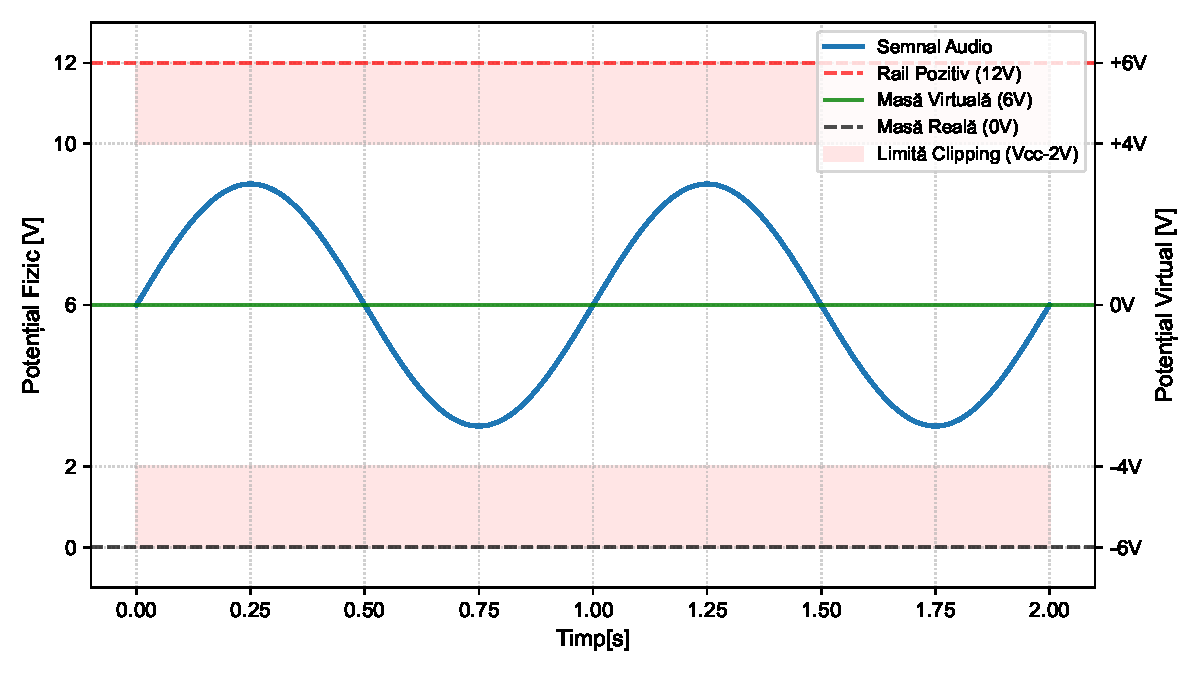
\includegraphics[width=0.9\textwidth]{figuri/virtual_ground_concept.pdf}
    \caption{Reprezentarea conceptuală a masei virtuale și a translației nivelurilor de tensiune.}
    \label{fig:virtual_ground_concept}
\end{figure}

Această translație definește intervalul teoretic de operare. Totuși, în practică, limita de tăiere (\textit{clipping}) a semnalului este impusă de limitările etajelor de ieșire ale amplificatoarelor operaționale. Deoarece componentele utilizate nu sunt de tip \textit{rail-to-rail}, tensiunea de ieșire nu poate atinge limitele șinelor de alimentare ($0\text{ V}$ și $12\text{ V}$), pragul de saturație apărând cu aproximativ $1.5\text{--}2\text{ V}$ înainte de aceste extreme. Astfel, dinamica reală a semnalului este limitată la un interval de aproximativ $8\text{ V}_{pp}$ (între $2\text{ V}$ și $10\text{ V}$ față de masa reală).

\subsection{Implementarea hardware a masei virtuale}
Circuitul utilizat pentru generarea referinței este prezentat în Figura \ref{fig:vgnd_sch}. Acesta utilizează un divizor de tensiune rezistiv ($R_1 = R_2 = 100\text{ k}\Omega$) pentru a minimiza consumul din sursa de alimentare. Punctul de mijloc al divizorului este urmat de un buffer cu un amplificator operațional \textbf{TL072} configurat ca repetor de tensiune.

\begin{figure}[htbp]
    \centering
    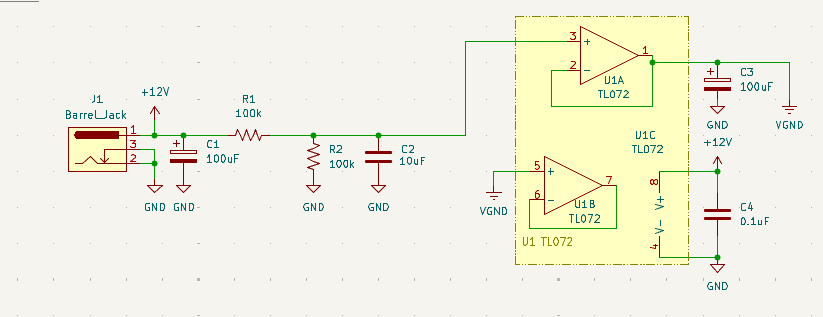
\includegraphics[width=0.9\textwidth]{figuri/schema_masa_virtuala.png}
    \caption{Schema electronică a sistemului de masă virtuală.}
    \label{fig:vgnd_sch}
\end{figure}

Buffer-ul implementat cu prima secțiune a amplificatorului operațional ($U_{1A}$) este esențial pentru a asigura o impedanță de ieșire scăzută a referinței de masă virtuală. Condensatorul $C_2$ îndeplinește rolul de decuplare a punctului de referință, furnizând o tensiune curată la intrarea ne-inversoare. Condensatorul electrolitic $C_1$ asigură filtrarea principală a sursei de alimentare, în timp ce $C_3$ acționează ca o rezervă locală de energie pentru a menține stabilitatea $V_{GND}$ în regim tranzitoriu. Suplimentar, s-a prevăzut utilizarea condensatorului ceramic $C_4$ ($0.1\text{ }\mu\text{F}$), plasat cât mai aproape de pinii de alimentare ai circuitului integrat $U_1$, cu rol de decuplare locală în înaltă frecvență pentru a preveni instabilitățile și a minimiza interferențele electromagnetice.

\subsection{Convertor DC-DC}
Deoarece procesorul digital de semnal (DSP) funcționează la un nivel de tensiune inferior etajelor analogice, s-a integrat un modul de conversie coborâtor (Buck converter) de tip \textbf{LM2596}. Acesta primește tensiunea principală de $12\text{ V}$ de la intrare și furnizează o tensiune stabilizată de $5\text{ V}$, dedicată exclusiv alimentării procesorului ADAU1701 și a logicii de control asociate. Utilizarea unui convertor în comutație în locul unui regulator liniar a fost preferată pentru a maximiza eficiența energetică și a minimiza disiparea termică în interiorul carcasei. Conexiunile acestui modul sunt prezentate în Figura \ref{fig:dcdc_sch}.

\begin{figure}[H]
    \centering
    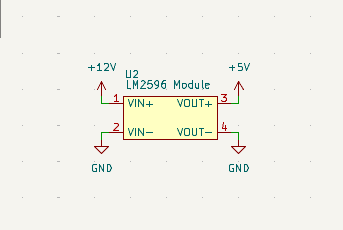
\includegraphics[width=0.5\textwidth]{figuri/DCDC.png}
    \caption{Reprezentarea conexiunilor modulului convertor DC-DC.}
    \label{fig:dcdc_sch}
\end{figure}

\section{Interfața de intrare de linie}
Etajul de intrare a fost implementat printr-o abordare hibridă, integrând suportul pentru semnale echilibrate (balanced) și neechilibrate (unbalanced) într-o structură unică. Această metodologie de proiectare reprezintă o sinteză a trei configurații arhitecturale fundamentale descrise de Douglas Self în \cite[Capitolul \textit{Line Inputs}]{douglasself}: \textit{A Practical Balanced Input}, \textit{Combined Unbalanced and Balanced Inputs} și \textit{Switched-Gain Balanced Inputs}.

\begin{figure}[htbp]
    \centering
    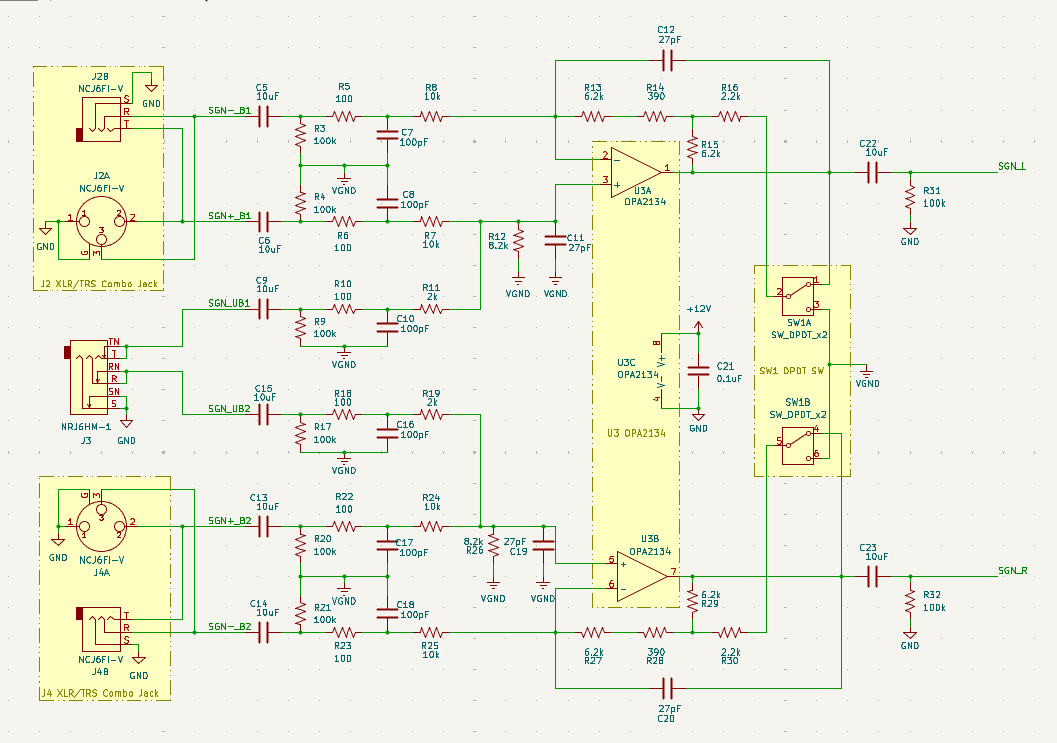
\includegraphics[width=0.9\textwidth]{figuri/Input_amp.png}
    \caption{Interfața de intrare de linie proiectată.}
    \label{fig:input_sch}
\end{figure}

\subsection{Integrarea conexiunilor echilibrate și neechilibrate}
Nucleul interfeței este constituit dintr-un amplificator diferențial realizat cu amplificatorul operațional \textbf{OPA2134}, recunoscut pentru densitatea scăzută a zgomotului ($8\text{ nV}/\sqrt{\text{Hz}}$). Pornind de la o topologie echilibrată standard (\textit{A Practical Balanced Input}), designul a fost extins prin adăugarea unei rute de semnal adiționale direct la intrarea ne-inversoare a operaționalului, conform principiului \textit{Combined Unbalanced and Balanced Inputs}. 

Această topologie permite utilizarea unei singure căi active de semnal pentru ambele standarde de conexiune, eliminând necesitatea unor comutatoare mecanice de selecție pe panoul frontal sau a unui etaj separat. În cazul unui semnal echilibrat (primit prin pinii XLR sau TRS ai conectorilor Combo J2/J4), circuitul amplifică diferența de potențial dintre ramura pozitivă și cea negativă. Pentru o sursă neechilibrată (primită prin pinul TS al conectorului J3), semnalul este aplicat doar pe intrarea dedicată, în timp ce ramura negativă a amplificatorului rămâne neconectată.

Literatura de specialitate avertizează însă asupra unui compromis inerent al acestei topologii \cite{douglasself}: performanța de zgomot în modul neechilibrat este ușor inferioară în comparație cu un etaj proiectat exclusiv pentru surse neechilibrate. Acest lucru se datorează faptului că rețeaua rezistivă din bucla de reacție a amplificatorului operațional (ex. R8, R15 etc.) rămâne în circuit, adăugând un nivel de zgomot termic Johnson-Nyquist adițional.

Zgomotul Johnson-Nyquist este generat de agitația termică a purtătorilor de sarcină din interiorul unui conductor electric, fiind direct proporțional cu temperatura absolută și cu valoarea rezistenței, aspect descris de ecuația fundamentală:
\begin{equation}
    V_n = \sqrt{4 k_B T R \Delta f}
\end{equation}
unde mărimile fizice implicate sunt \cite{douglasself}:
\begin{itemize}
    \item $V_n$ -- tensiunea efectivă a zgomotului termic ($\text{V}_{rms}$);
    \item $k_B$ -- constanta lui Boltzmann ($\approx 1.38 \times 10^{-23}\text{ J/K}$);
    \item $T$ -- temperatura absolută a conductorului ($\text{K}$);
    \item $R$ -- rezistența electrică ($\Omega$);
    \item $\Delta f$ -- lățimea de bandă de măsură ($\text{Hz}$).
\end{itemize}

Mai mult, impedanța de intrare pe calea neechilibrată nu poate fi proiectată arbitrar de mare, fiind influențată de valorile rezistențelor din rețeaua diferențială. De asemenea, este foarte important ca doar una dintre cele două intrări (echilibrată sau neechilibrată) să fie utilizată la un moment dat. Dacă s-ar conecta o sursă neechilibrată în timp ce conexiunea echilibrată este activă, s-ar crea o buclă de masă care ar induce zgomot nedorit. 

\subsection{Filtrarea și condiționarea semnalului}
Pentru a asigura funcționarea stabilă într-un mediu predispus la interferențe electromagnetice, fiecare intrare este prevăzută cu un filtru trece-jos pentru radiofrecvență. Acesta este compus dintr-o rețea RC pasivă, cu valorile $R = 100\text{ }\Omega$ (R5) și $C = 100\text{ pF}$ (C7). Frecvența de tăiere a acestui filtru a fost calculată astfel:
\begin{equation}
    f_{c_{RFI}} = \frac{1}{2\pi R C} \approx 15.9\text{ MHz}
\end{equation}

Izolarea în curent continuu este realizată în două etape. La intrarea etajului, condensatoarele de $10\text{ }\mu\text{F}$ formează un filtru trece-sus cu următoarea frecvență de tăiere inferioară:
\begin{equation}
    f_{HPF,in} = \frac{1}{2\pi Z_{in} C_c} \approx 1.59\text{ Hz}
\end{equation}

Suplimentar, la ieșirea interfeței de intrare, s-a implementat un al doilea filtru trece-sus format din condensatorul $C_{22} = 10\text{ }\mu\text{F}$ și rezistența $R_{31} = 100\text{ k}\Omega$ conectată la masă. Rolul critic al acestui filtru este eliminarea componentei continue de tip masă virtuală ($V_{GND} = 6\text{ V}$) din semnalul analogic prelucrat. Această decuplare este obligatorie pentru a permite cuplarea corectă a semnalului audio către pinii de intrare ai procesorului DSP, care necesită o referință de curent continuu diferită. Frecvența de tăiere a acestui etaj de decuplare este extrem de joasă pentru a nu afecta faza semnalului:
\begin{equation}
    f_{HPF,out} = \frac{1}{2\pi R_{31} C_{22}} = \frac{1}{2\pi \cdot 100\text{ k}\Omega \cdot 10\text{ }\mu\text{F}} \approx 0.16\text{ Hz}
\end{equation}

\subsection{Comutarea câștigulului }
Sistemul trebuie să asigure alinierea nivelurilor de semnal provenite de la surse cu standarde diferite: echipamente profesionale ($+4\text{ dBu} \approx 1.228\text{ V}_{rms}$) și echipamente de consum ($-10\text{ dBV} \approx 0.316\text{ V}_{rms}$). Pentru a optimiza gama dinamică a DSP-ului, etajul de intrare utilizează o tehnică avansată numită \textit{Switched-Gain Balanced Input}, documentată de Douglas Self \cite{douglasself}.

Spre deosebire de metodele brute care comută valorile rezistențelor principale de intrare sau reacție necesitând comutatoare multiple și riscând degradarea CMRR prin asimetrii, această metodă manipulează doar semnalul care alimenteaza brațul de reacție. Principiul fundamental constă în menținerea unei impedanțe de sursă constante pentru brațul de reacție, indiferent de poziția comutatorului, asigurând astfel că raportul dintre brațele amplificatorului diferențial rămâne echilibrat.

Configurația utilizată (Figura \ref{fig:input_sch}) se bazează pe rețeaua formată din $R_{15} = 6.2\text{ k}\Omega$ și $R_{16} = 2.2\text{ k}\Omega$. Impedanța de sursă văzută de brațul de reacție este dată de paralelul acestora:
\begin{equation}
    Z_{s,fb} = R_{15} \parallel R_{16} = \frac{6.2\text{ k}\Omega \cdot 2.2\text{ k}\Omega}{6.2\text{ k}\Omega + 2.2\text{ k}\Omega} \approx 1.624\text{ k}\Omega
\end{equation}
Această valoare rămâne constantă deoarece, din perspectiva nodului de reacție, atât ieșirea amplificatorului operațional (în modul \textit{Low Gain}), cât și masa (în modul \textit{High Gain}), prezintă o impedanță efectiv nulă. 

Pentru a menține CMRR-ul maxim, rezistența totală a brațului de reacție trebuie să fie egală cu rezistența brațului ne-inversor ($R_{12} = 8.2\text{ k}\Omega$). Brațul de reacție este compus din suma $R_{13} + R_{14}$ plus impedanța de sursă $Z_{s,fb}$:
\begin{equation}
    R_{fb,total} = R_{13} + R_{14} + Z_{s,fb} = 6.2\text{ k}\Omega + 390\text{ }\Omega + 1.624\text{ k}\Omega = 8.214\text{ k}\Omega
\end{equation}
Eroarea de doar $14\text{ }\Omega$ față de valoarea țintă de $8.2\text{ k}\Omega$ este sub pragul de toleranță de $1\%$ al rezistențelor utilizate, având un efect neglijabil asupra performanței CMRR.

\textbf{1. Regimul \textit{Low Gain} (+4dBu)} \\
În această poziție, $R_{16}$ este conectat la ieșirea op-amp-ului, semnalul de reacție nefiind atenuat. Câștigul este determinat de raportul dintre rezistența de reacție și cea de intrare ($R_7, R_8 = 10\text{ k}\Omega$):
\begin{equation}
    G_{low} = \frac{R_{fb,total}}{R_{7}} = \frac{8.214\text{ k}\Omega}{10\text{ k}\Omega} \approx 0.82
\end{equation}
Pentru un semnal profesional de intrare de $+4\text{ dBu}$ ($1.228\text{ V}_{rms}$), tensiunea la ieșirea etajului este atenuată la:
\begin{equation}
    V_{out,low} = 1.228\text{ V}_{rms} \cdot 0.82 \approx 1.007\text{ V}_{rms}
\end{equation}

\textbf{2. Regimul \textit{High Gain} (-10dBV)} \\
Prin comutarea $R_{16}$ la masă, $R_{15}$ și $R_{16}$ formează un divizor de tensiune care scalează ieșirea. Factorul de multiplicare al câștigului este dat de atenuarea acestui divizor:
\begin{equation}
    G_{high} = G_{low} \cdot \left( 1 + \frac{R_{15}}{R_{16}} \right) = 0.82 \cdot \left( 1 + \frac{6.2\text{ k}\Omega}{2.2\text{ k}\Omega} \right) \approx 3.13
\end{equation}
Pentru un semnal de nivel \textit{consumer} de $-10\text{ dBV}$ ($0.316\text{ V}_{rms}$), tensiunea la ieșirea etajului este amplificată la:
\begin{equation}
    V_{out,high} = 0.316\text{ V}_{rms} \cdot 3.13 \approx 0.989\text{ V}_{rms}
\end{equation}

Astfel, ambele standarde de intrare sunt mapate eficient la nivelul țintă de aproximativ $1\text{ V}_{rms}$, optim pentru prelucrarea ulterioară în DSP.

\subsection{Simularea SPICE a etajului de intrare}
Validarea topologiei a fost efectuată prin analize SPICE.

\subsubsection{Analiza în regim tranzitoriu și maparea nivelurilor}
S-a efectuat o analiză tranzitorie cu semnale sinusoidale la $1\text{ kHz}$ pentru verificarea preciziei etajului de adaptare a câștigului. Scopul este demonstrarea faptului că standardele de intrare (+4 dBu profesional și -10 dBV consumer) sunt scalate la nivelul de $1\text{ V}_{rms}$.

Figurile \ref{fig:input_transient} centralizează rezultatele simulării pentru cele patru scenarii de operare:
\begin{itemize}
    \item \textbf{Mod Echilibrat / Neechilibrat (Câștig Scăzut):} Un semnal de intrare de calibrare profesională (+4 dBu), având o valoare măsurată de aproximativ $1.228\text{ V}_{rms}$ este atenuat de etajul analogic. Ieșirea rezultată este menținută la nivelul calculat teoretic de $\approx 1.007\text{ V}_{rms}$.
    \item \textbf{Mod Echilibrat / Neechilibrat (Câștig Ridicat):} Un semnal de nivel consumer (-10 dBV), măsurând aproximativ $0.316\text{ V}_{rms}$, este amplificat de etajul analogic la nivelul de $\approx 0.989\text{ V}_{rms}$.
\end{itemize}

\begin{figure}[htbp]
    \centering
    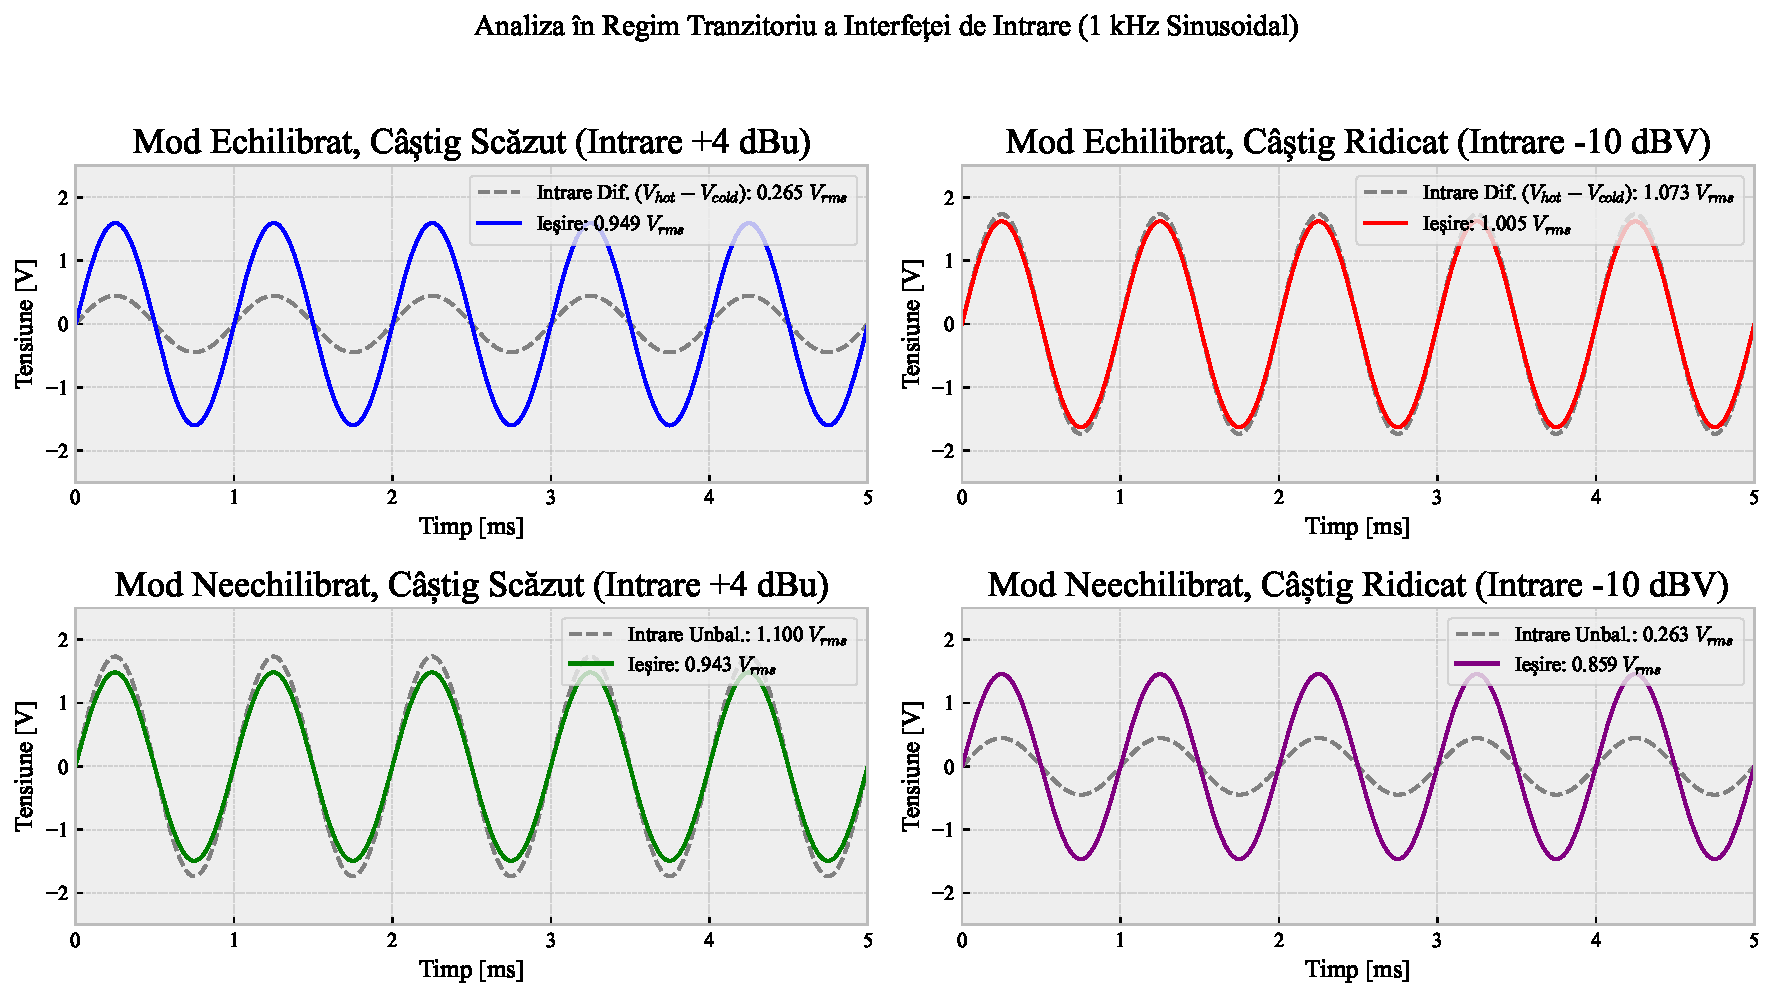
\includegraphics[width=0.85\textwidth]{figuri/input_transient.pdf}
    \caption{Simularea mapării nivelurilor de intrare (+4 dBu și -10 dBV) la nivelul de 1 Vrms. Sunt ilustrate cele patru scenarii posibile de interconectare (Echilibrat/Neechilibrat $\times$ Low/High Gain).}
    \label{fig:input_transient}
\end{figure}

Extragerea valorilor RMS direct din semnalele tranzitorii validate confirmă precizia designului hibrid. Această aliniere este critică pentru a asigura utilizarea optimă a gamei dinamice a convertorului analog-digital (ADC) al procesorului ADAU1701. Deoarece pragul absolut de saturație digitală (\textit{clipping}) al ADC-ului este de $2\text{ V}_{rms}$, maparea controlată la $1\text{ V}_{rms}$ garantează un \textit{headroom} de exact $6\text{ dB}$, protejând sistemul în timpul pasajelor audio dinamice.

\subsubsection{Răspunsul în frecvență și faza}

\begin{figure}[H]
	\centering
	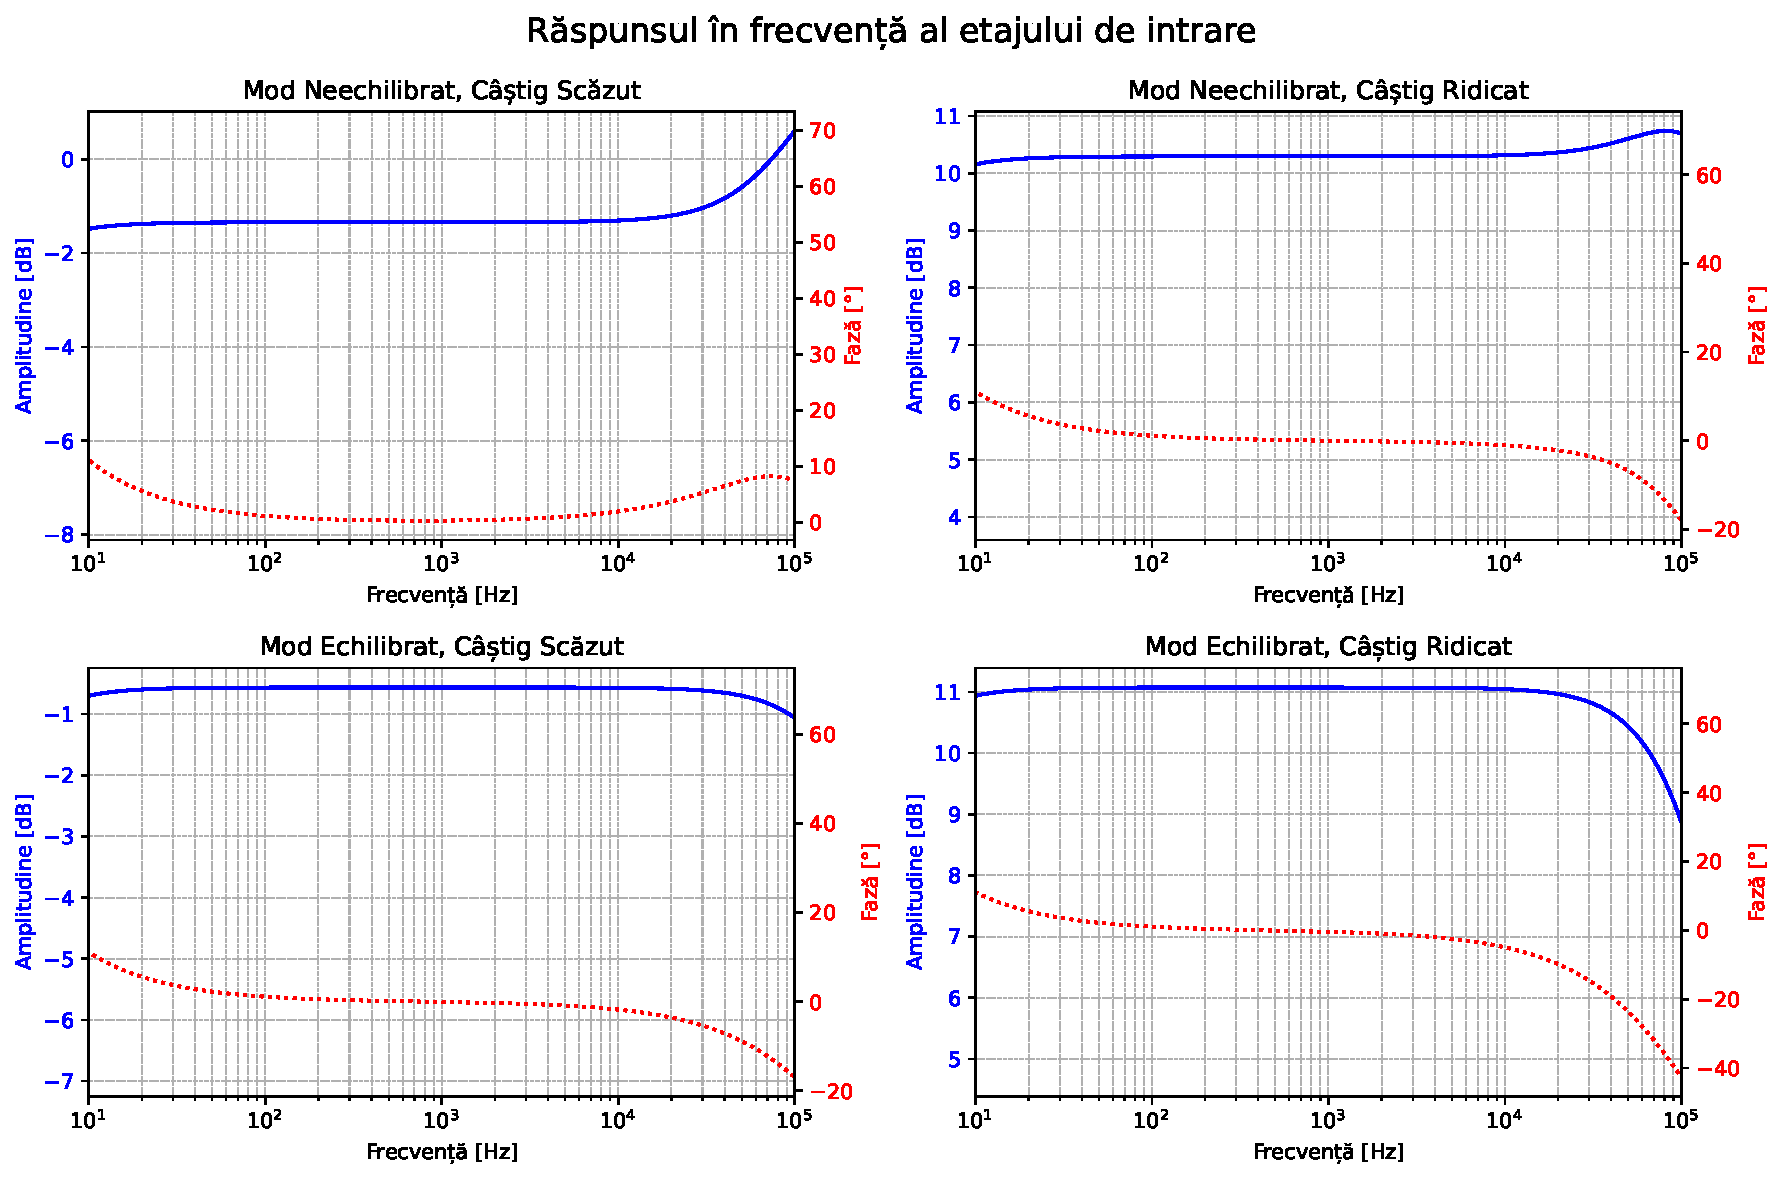
\includegraphics[width=0.85\textwidth]{figuri/freq_resp_input.pdf}
	\caption{Răspunsul în frecvență (amplitudine și fază) al etajului de intrare, simulat în AC (1 Hz - 100 kHz).}
	\label{fig:input_freq_resp}
\end{figure}

Graficele indică un răspuns constant în amplitudine, în spectrul audio de interes (20 Hz - 20 kHz), pentru fiecare configurație în parte. Faza rămâne liniară în această regiune, abaterile la frecvențe foarte joase fiind atribuite condensatoarelor de decuplare utilizate pe intrări. Aceste rezultate atestă stabilitatea și performanța etajului în tratarea semnalelor de intrare variate.


\subsubsection{Analiza impedanței}
O caracteristică importantă a interfețelor de linie este impedanța de intrare. Rezultatele simulării pentru modul echilibrat indică o asimetrie între ramuri (Figura \ref{fig:input_impedance}).

\begin{figure}[htbp]
    \centering
    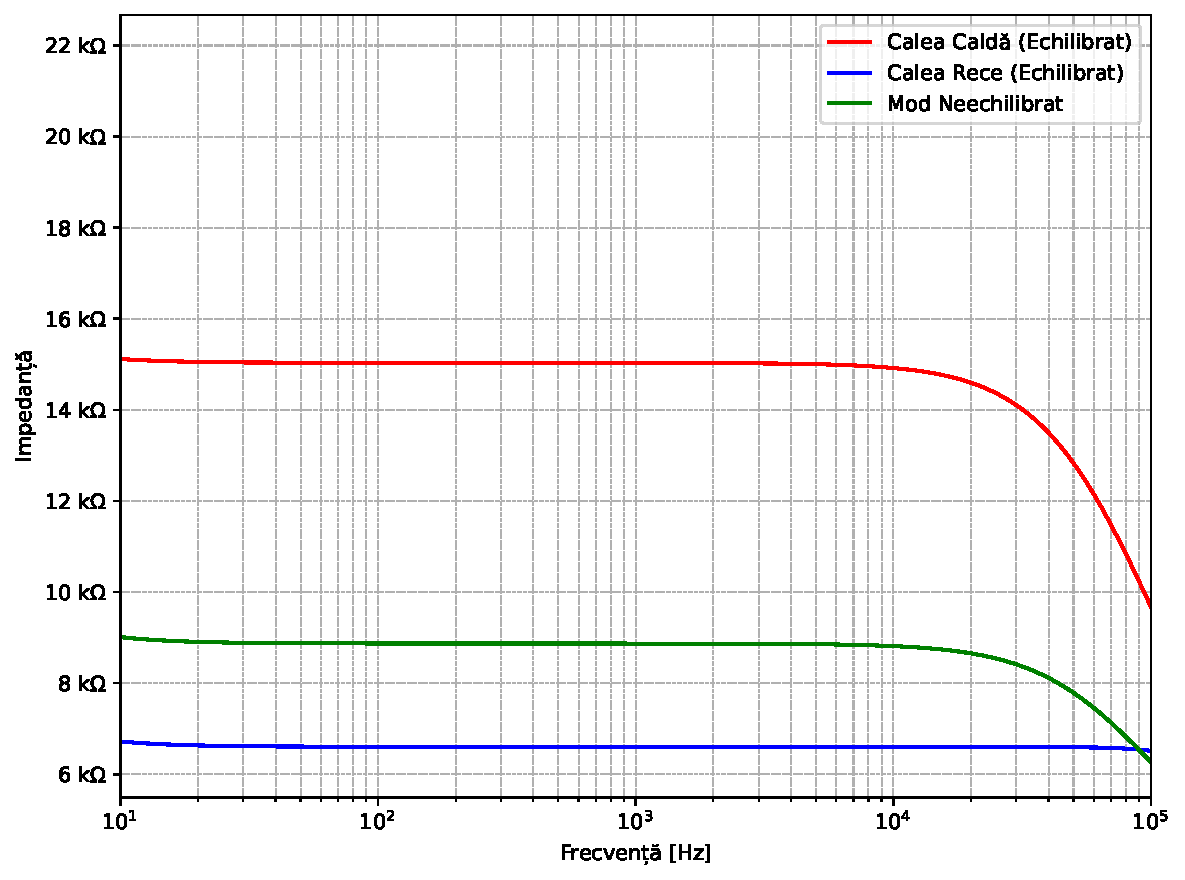
\includegraphics[width=0.85\textwidth]{figuri/input_impedance.pdf}
    \caption{Magnitudinea impedanței de intrare în funcție de frecvență.}
    \label{fig:input_impedance}
\end{figure}

Calculul teoretic explică valorile de aproximativ $15\text{ k}\Omega$ pentru ramura \textit{Caldă} și $7\text{ k}\Omega$ pentru cea \textit{Rece}. Pentru ramura \textit{Rece} (conectată la intrarea inversoare prin rezistența $R_8$), apare fenomenul de \textbf{anti-bootstrapping} \cite{douglasself}. Deoarece amplificatorul operațional menține un scurtcircuit virtual între intrările sale ($V_- = V_+$), tensiunea la nodul inversor ($V_-$) o urmărește pe cea de la nodul ne-inversor ($V_+$). Tensiunea $V_+$ este dictată de divizorul rezistiv format din $R_{7}$ și $R_{12}$, acesta fiind alimentat de semnalul aplicat pe ramura \textit{Caldă}.

Într-o conexiune echilibrată, semnalele sunt în antifază ($V_{rece} = -V_{cald}$). Astfel, la capătul rezistenței $R_8$ dinspre amplificatorul operațional ($V_-$) va exista o tensiune de polaritate opusă celei aplicate la intrarea \textit{Rece}. Acest lucru determină o cădere de tensiune mai mare pe $R_8$ decât dacă $V_-$ ar fi fost conectat la masă, generând un curent absorbit crescut și, în consecință, o impedanță de intrare diminuată:
\begin{equation}
    Z_{in,rece} = R_3 \parallel \frac{R_8 +R5}{1 + \frac{R_{12}}{R_7 + R_{12}}} =100\text{ k}\Omega \parallel \frac{10.1\text{ k}\Omega}{1 + \frac{8.2\text{ k}\Omega}{10\text{ k}\Omega + 8.2\text{ k}\Omega}} \approx \frac{10.1\text{ k}\Omega}{1.45} \approx 6.9\text{ k}\Omega
\end{equation}

Pentru ramura \textit{Caldă}, impedanța este determinată de rețeaua pasivă de la intrarea ne-inversoare:
\begin{equation}
    Z_{in,cald} \approx R_4 \parallel (R_{5} + R_{7} + R_{12}) = 100\text{ k}\Omega \parallel (100\text{ }\Omega + 10\text{ k}\Omega + 8.2\text{ k}\Omega) \approx 15.4\text{ k}\Omega
\end{equation}

Pentru intrarea neechilibrată, impedanța de intrare se calculează astfel:
\begin{equation}
    Z_{in,unbal} = R_9 \parallel (R_{10} + R_{11} + R_{12}) = 100\text{ k}\Omega \parallel (100\text{ }\Omega + 2\text{ k}\Omega + 8.2\text{ k}\Omega) \approx 9.3\text{ k}\Omega
\end{equation}

Această asimetrie a impedanțelor de intrare este o trăsătură inerentă a topologiei de amplificator diferențial cu un singur amplificator operațional. Totuși, așa cum demonstrează Douglas Self, asimetria se manifestă exclusiv pentru semnalele diferențiale. Rejecția modului comun (CMRR) depinde strict de egalitatea impedanțelor pentru semnalele de mod comun. Deoarece zgomotele induse pe cablu sunt identice pe ambele ramuri ($V_{cald} = V_{rece}$), fenomenul de anti-bootstrapping nu are loc, iar impedanțele de intrare în mod comun devin complet egale, permițând obținerea unui CMRR nedegradat \cite{douglasself}.

\section{Procesorul Digital de Semnal}
Inima sistemului de procesare este constituită de un modul bazat pe procesorul de semnal ADAU1701, produs de Analog Devices. Alegerea acestui DSP a fost motivată de arhitectura sa integrată (\textit{single-chip}), care include două convertoare analog-digitale (ADC) și patru convertoare digital-analogice (DAC). Această configurație hardware cu 2 intrări și 4 ieșiri este ideală pentru implementarea filtrelor de tip \textit{crossover} (separare în frecvență) necesare unui sistem multicanal.

Așa cum a fost detaliat în analiza etajului de intrare, semnalul audio aplicat la pinii ADC-ului a fost condiționat la o valoare nominală de aproximativ $1\text{ V}_{rms}$. Având în vedere că nivelul maxim acceptat de convertoarele integrate înainte de saturația digitală (\textit{clipping}) este de $2\text{ V}_{rms}$, semnalul va opera la un nivel nominal de $\approx -6\text{ dBFS}$ (decibeli față de capătul de scală -- \textit{Full Scale}). Această alegere strategică asigură un \textit{headroom} (rezervă de dinamică) de $6\text{ dB}$.
\begin{figure}[htbp]
    \centering
    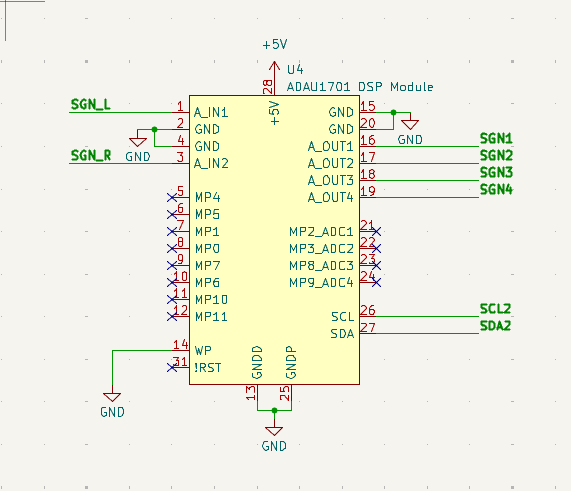
\includegraphics[width=0.7\textwidth]{figuri/schema_dsp.png}
    \caption{Integrarea modulului DSP ADAU1701 în circuit.}
    \label{fig:dsp_sch}
\end{figure}

\section{Programatorul DSP și Interfața de Control}
Pentru a permite comunicarea în timp real între mediul de dezvoltare SigmaStudio și procesorul ADAU1701, a fost integrat un modul de programare dedicat. Acesta este realizat utilizând o placă de dezvoltare cu microcontrolerul USB \textbf{CY7C68013A}. Construcția și adaptarea acestui modul s-au bazat pe instrucțiunile și topologia proiectului open-source \textit{freeUSBi} \cite{freeusbi}.

\begin{figure}[htbp]
    \centering
    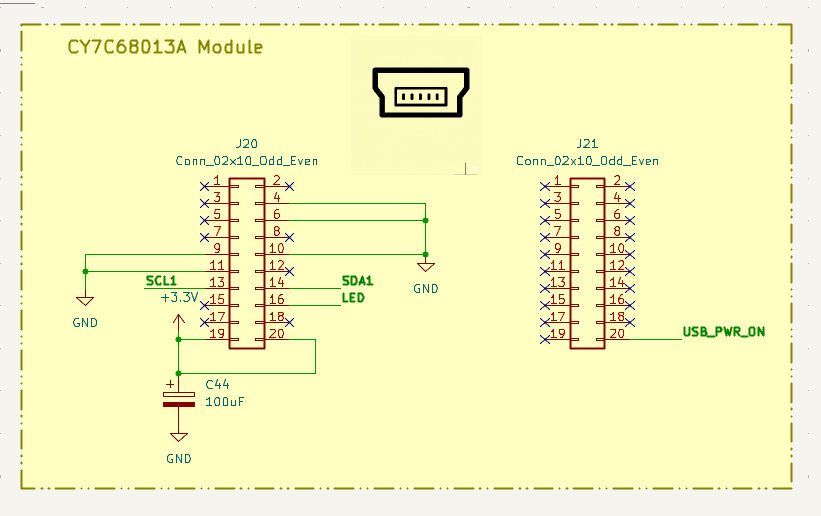
\includegraphics[width=0.7\textwidth]{figuri/schema_programator.png}
    \caption{Schema modulului de programare USB bazat pe CY7C68013A.}
    \label{fig:schema_prog}
\end{figure}

Pe lângă modulul USB propriu-zis, sistemul include un circuit auxiliar de izolare a magistralei (\textit{bus isolator}), prezentat în Figura \ref{fig:bus_iso}. Acest circuit este format din două tranzistoare MOSFET care au rolul de a izola și comanda liniile magistralei $\text{I}^2\text{C}$ ($SDA$ și $SCL$) prin care se programează DSP-ul. Izolarea previne blocarea magistralei sau interferențele în timpul în care programatorul nu este conectat la PC. De asemenea, circuitul include un LED indicator care semnalizează vizual momentul în care are loc transferul de date (programarea efectivă).

\begin{figure}[ht]
    \centering
    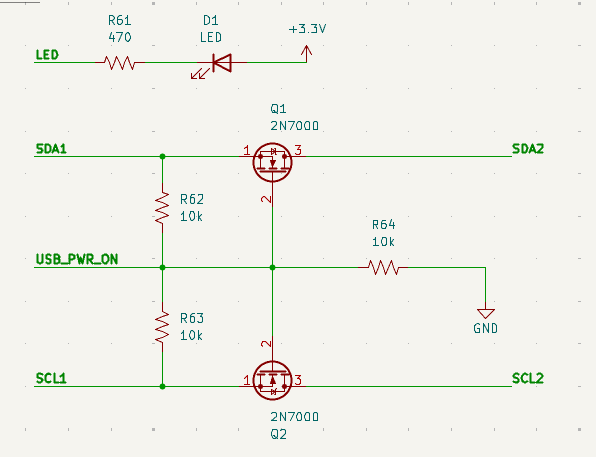
\includegraphics[width=0.6\textwidth]{figuri/bus_iso.png}
    \caption{Circuitul de izolare a magistralei I2C și indicatorul de programare.}
    \label{fig:bus_iso}
\end{figure}

Din punct de vedere software, recunoașterea programatorului de către sistemul de operare și integrarea sa cu mediul SigmaStudio necesită instalarea unui driver USB custom (\textit{cyusb3.sys}). Acest driver, împreună cu restul resurselor, a fost documentat și distribuit de inițiativa \textit{freeUSBi} \cite{freeusbi}.

\section{Etajele de putere în clasa D}
Pentru a asigura acționarea directă a difuzoarelor, sistemul integrează patru module de amplificare de putere în clasa D, bazate pe circuitul integrat \textbf{TPA3118}. Fiecare modul primește unul dintre cele patru semnale audio procesate și analogice provenite de la ieșirile DAC ale procesorului DSP.

Alegerea amplificatoarelor în clasa D a fost dictată de eficiența lor ridicată, care permite obținerea unei puteri considerabile fără necesitatea unor radiatoare de mari dimensiuni. La tensiunea de alimentare de $12\text{ V}$ utilizată în acest proiect, modulele furnizează o putere suficientă pentru audiție de proximitate, iar ieșirile acestora sunt conectate direct la panoul posterior al dispozitivului prin intermediul unor terminale tip banană, asigurând o conexiune robustă și fiabilă cu boxele.

\begin{figure}[H]
    \centering
    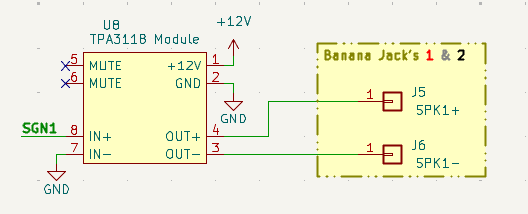
\includegraphics[width=0.7\textwidth]{figuri/Damp.png}
    \caption{Schema de conectare a unui modul de amplificare TPA3118.}
    \label{fig:power_amp_sch}
\end{figure}

\section{Interfața de ieșire de linie}
Pentru a permite utilizarea sistemului într-un context audio profesional, unde este necesară interconectarea cu echipamente externe (mixere, monitoare active sau stații de amplificare externe), s-a proiectat o interfață de ieșire de linie echilibrată. Aceasta preia semnalele analogice furnizate de cele patru DAC-uri ale procesorului DSP. Este important de menționat că fiecare ieșire a DSP-ului este conectată în paralel atât către etajul intern de putere (clasa D), cât și către acest etaj de ieșire de linie.

\begin{figure}[H]
    \centering
    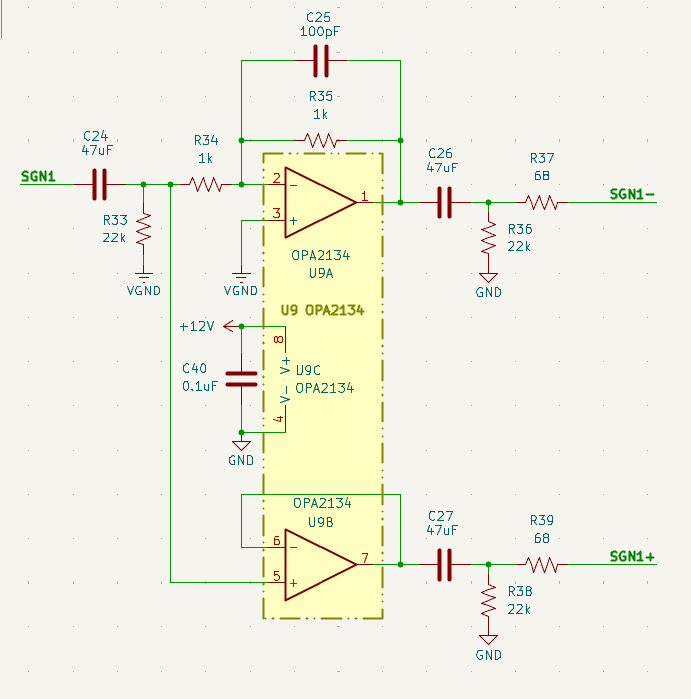
\includegraphics[width=0.7\textwidth]{figuri/output_amp.png}
    \caption{Schema electronică a etajului de ieșire echilibrat.}
    \label{fig:output_sch}
\end{figure}

Spre deosebire de configurația neechilibrată sau cea cu echilibrare pasivă, s-a ales o topologie de \textbf{ieșire echilibrată activă} (\textit{True Balanced Output}), similară celei prezentate în \cite{douglasself}. Această arhitectură asigură generarea unui semnal diferențial real, unde ramura negativă poartă semnalul în antifază.

\subsection{Analiza circuitului și selecția componentelor}
Nucleul interfeței este constituit din amplificatorul operațional dual \textbf{OPA2134}. Prima secțiune a acestuia ($U_{9B}$) este configurată ca repetor de tensiune (buffer), furnizând semnalul în fază pentru ramura pozitivă (\textit{Cald}). Cea de-a doua secțiune ($U_{9A}$) este configurată ca amplificator inversor cu câștig unitar, utilizând rezistențele $R_{34} = R_{35} = 1\text{ k}\Omega$ cu valori optime pentru un zgomot Johnson-Nyquist scăzut, pentru a genera semnalul în antifază pentru ramura negativă (\textit{Rece}).

Condensatorul de compensare $C_{25}$ ($100\text{ pF}$), plasat în bucla de reacție a etajului inversor, asigură stabilitatea amplificatorului la frecvențe înalte.

Condiționarea semnalului include următoarele elemente critice:
\begin{itemize}
    \item \textbf{Izolarea în curent continuu:} Condensatorul $C_{24}$ ($47\text{ }\mu\text{F}$) și rezistența $R_{33}$ ($22\text{ k}\Omega$) asigură polarizarea intrărilor la masa virtuală a sistemului.
    \item \textbf{Decuplarea ieșirii:} La ieșire, condensatoarele $C_{26}$ și $C_{27}$ ($47\text{ }\mu\text{F}$) blochează o componentă continuă, protejând echipamentele externe. Rezistențele $R_{36}$ și $R_{3B}$ ($22\text{ k}\Omega$) sunt conectate la masă pentru a elimina acumularea sarcinilor electrostatice pe pinii conectorilor, prevenind astfel zgomotele tranzitorii ("pocniturile") la cuplarea cablurilor.
    \item \textbf{Impedanța de ieșire și stabilitatea:} Rezistențele serie $R_{37}$ și $R_{39}$ ($68\text{ }\Omega$) definesc impedanța de ieșire a interfeței și oferă o protecție limitată la scurtcircuit accidental pe linii.
\end{itemize}

\subsection{Simularea performanțelor etajului de ieșire}
Validarea designului s-a realizat prin simulări SPICE, vizând regimul tranzitoriu, răspunsul în frecvență și impedanța de ieșire.

\subsubsection{Analiza în regim tranzitoriu}
Simularea tranzitorie a fost efectuată utilizând un semnal sinusoidal de test la frecvența de $1\text{ kHz}$. Rezultatele extrase din simulare confirmă funcționarea corectă a topologiei active. Pentru un semnal de intrare de referință, brațul \textit{Hot} repetă semnalul, în timp ce brațul \textit{Cold} generează un semnal identic în amplitudine, dar defazat cu $180^\circ$, așa cum este ilustrat în Figura \ref{fig:output_transient}.

\begin{figure}[H]
    \centering
    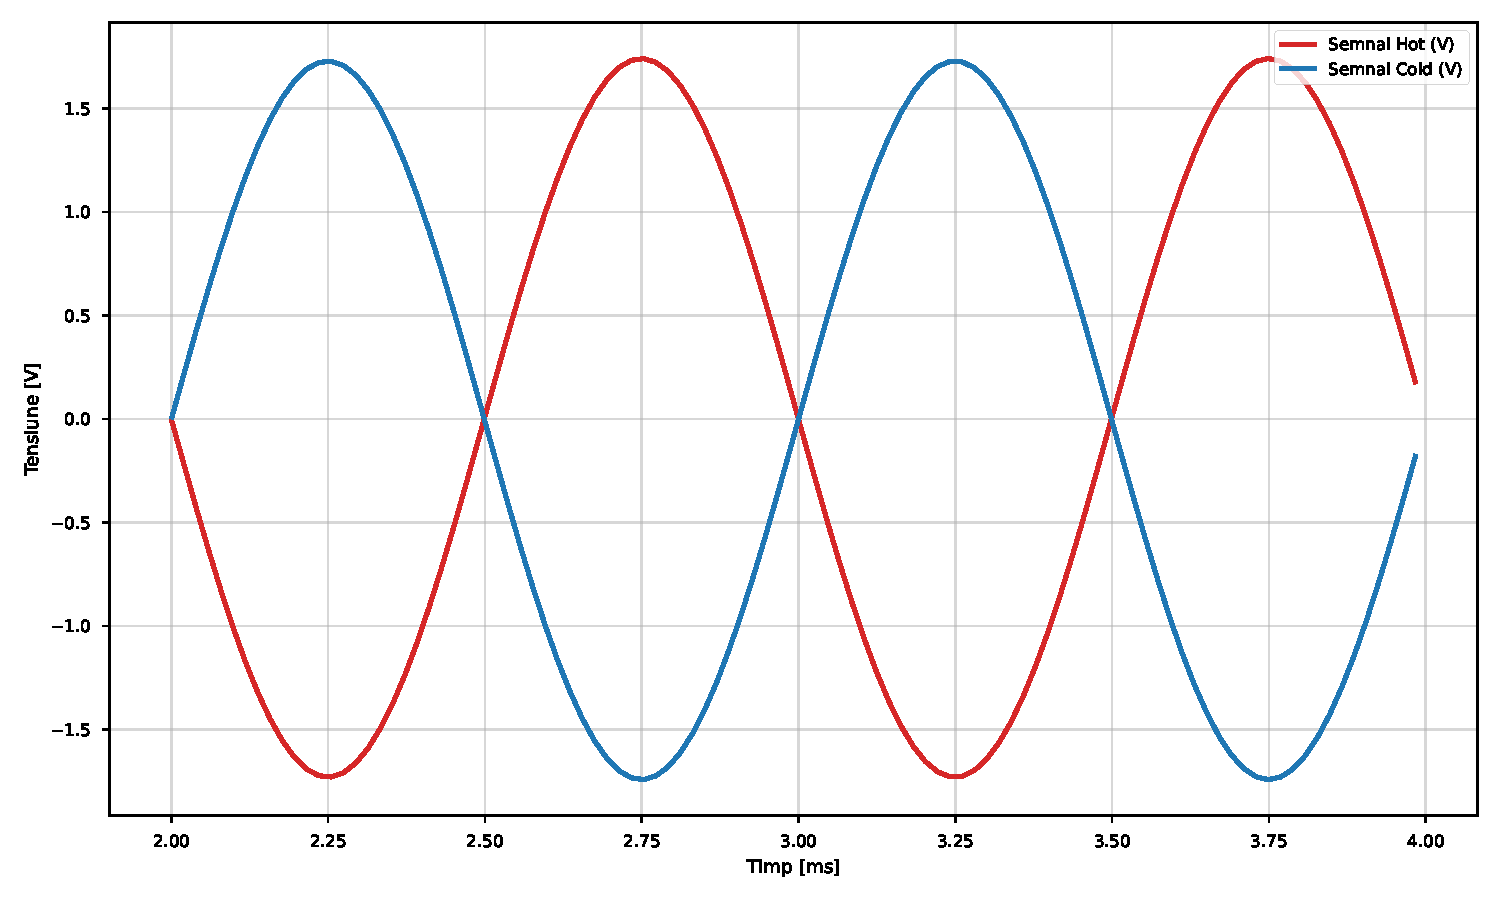
\includegraphics[width=0.75\textwidth]{figuri/output_transient.pdf}
    \caption{Simularea în regim tranzitoriu a interfeței de ieșire.}
    \label{fig:output_transient}
\end{figure}


\subsubsection{Răspunsul în frecvență}
Analiza în curent alternativ evidențiază un câștig unitar ($0\text{ dB}$) pe ambele ramuri în banda audio de interes. Graficul (Figura \ref{fig:output_freq_resp}) prezintă atât magnitudinea (sus), cât și faza semnalului (jos), confirmă liniaritatea răspunsului pentru ambele ramuri (Hot și Cold). Se observă o atenuare neglijabilă la frecvențe foarte joase, în timp ce faza rămâne liniară.

\begin{figure}[H]
    \centering
    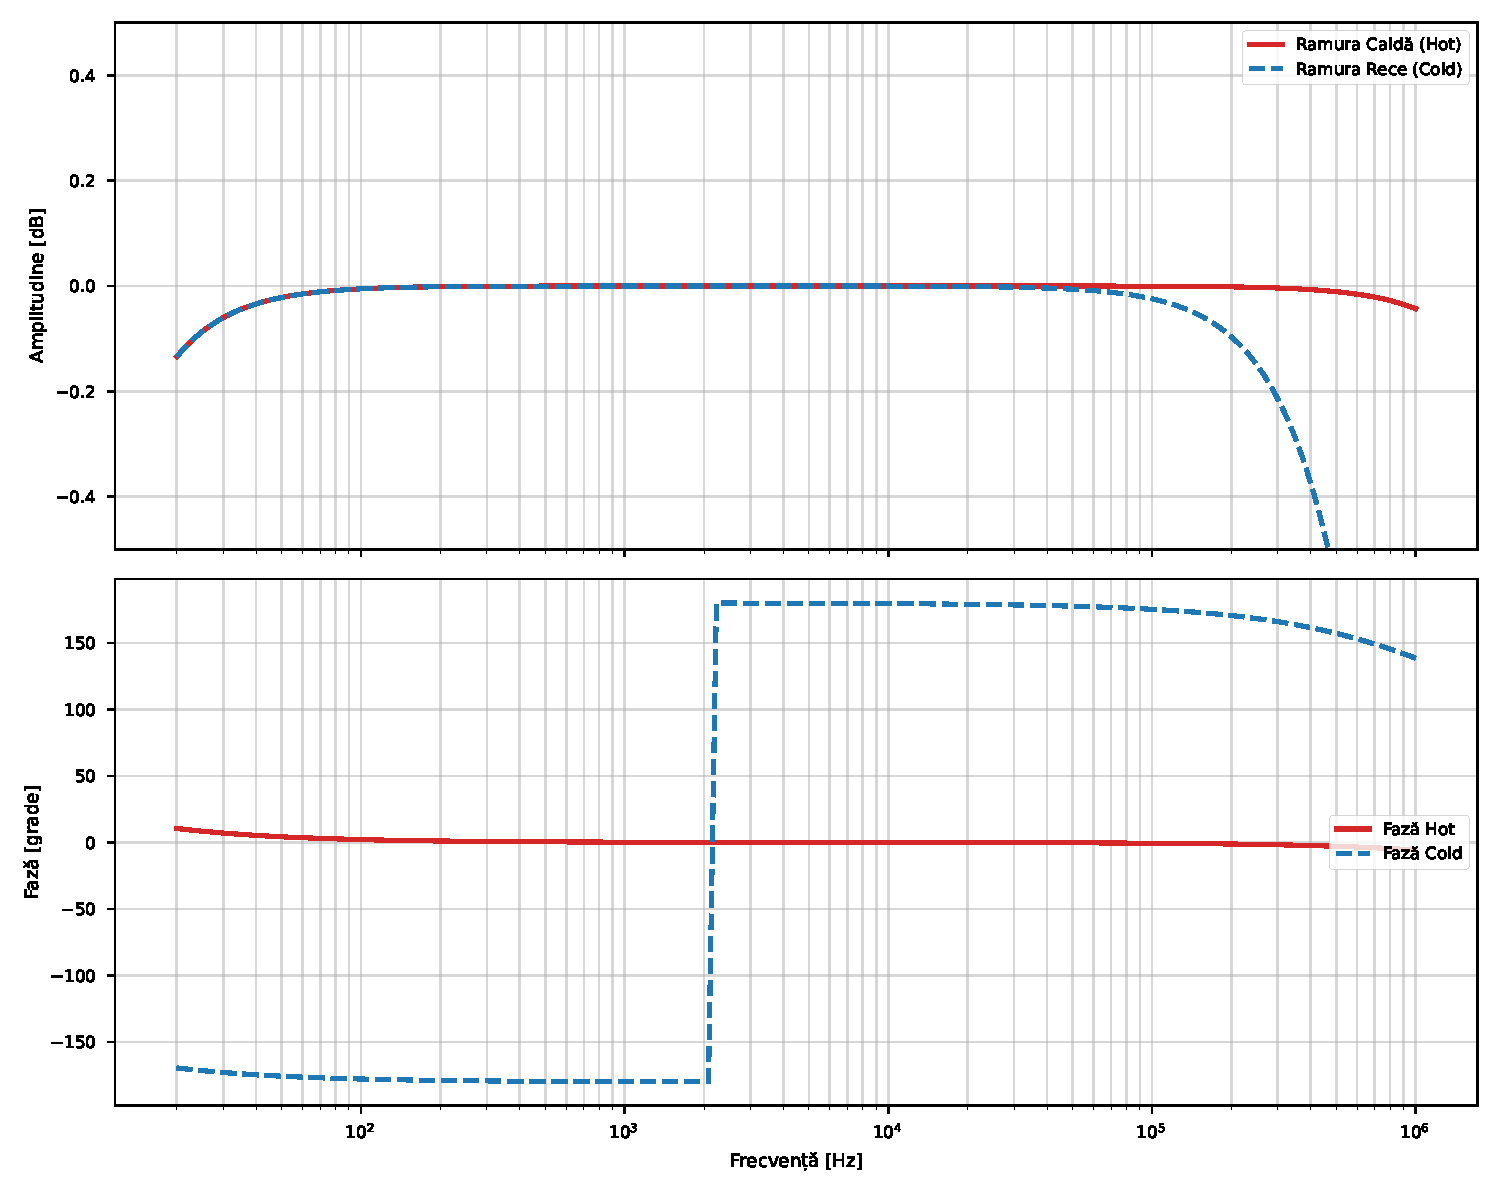
\includegraphics[width=0.7\textwidth]{figuri/freq_resp_output.pdf}
    \caption{Răspunsul în frecvență (magnitudine și fază) simulat pentru interfața de ieșire.}
    \label{fig:output_freq_resp}
\end{figure}

\subsubsection{Analiza impedanței de ieșire}
O condiție critică pentru o interfață echilibrată este simetria impedanțelor de ieșire. Rezultatele simulării (Figura \ref{fig:output_impedance}) confirmă acest aspect: ambele ramuri prezintă o impedanță constantă de aproximativ $68\text{ }\Omega$ în banda audio. Această simetrie este esențială pentru a asigura o rejecție ridicată a zgomotului de mod comun (CMRR) la destinație.

\begin{figure}[!ht]
    \centering
    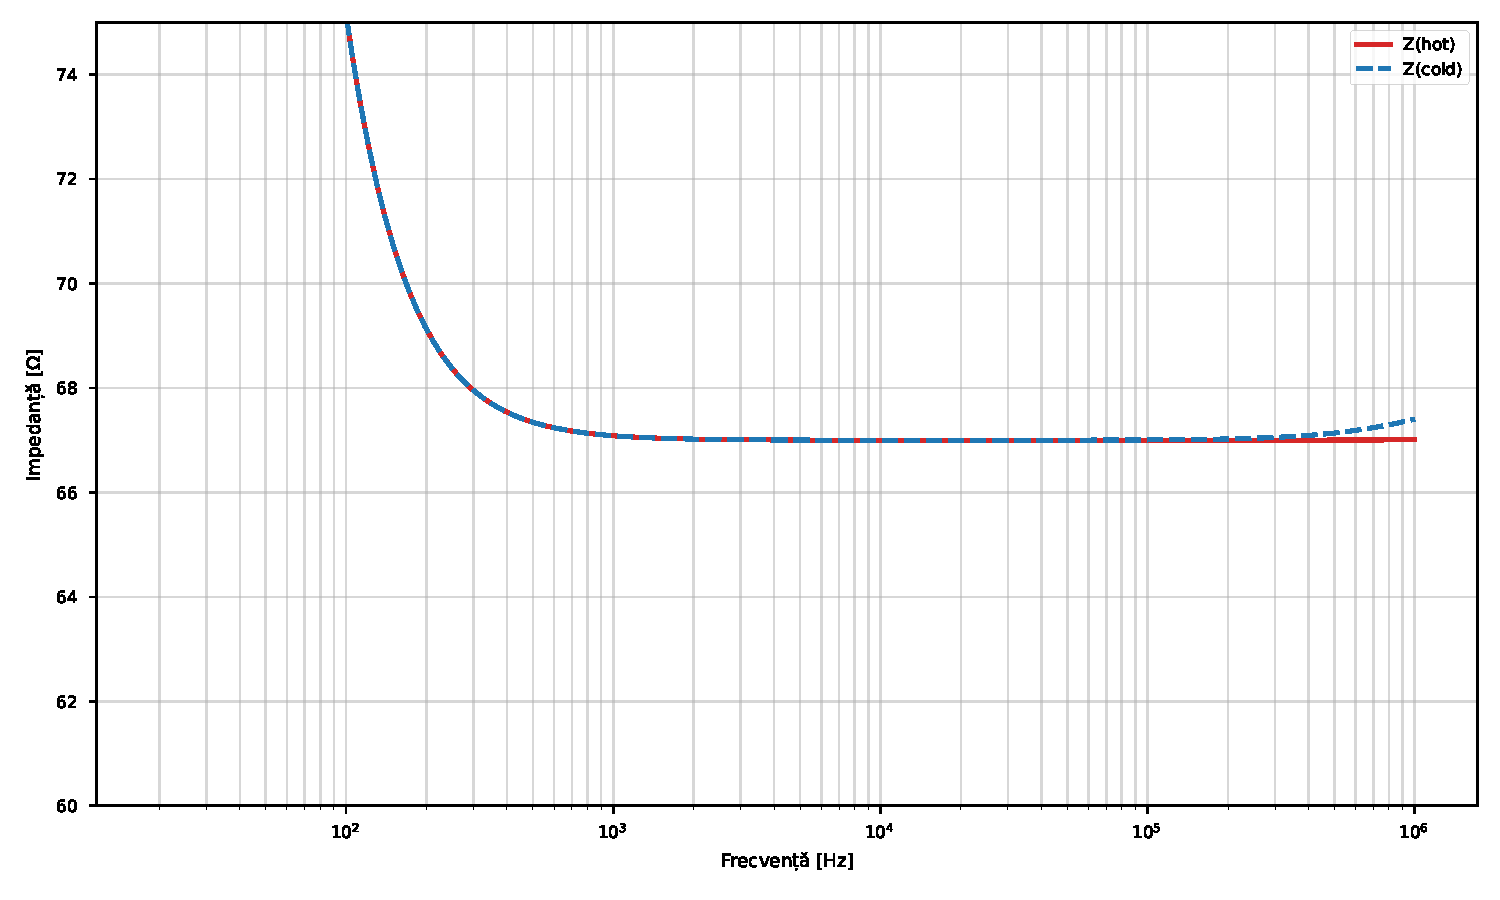
\includegraphics[width=0.7\textwidth]{figuri/output_impedance.pdf}
    \caption{Impedanța de ieșire simulată pentru ramurile Cald și Rece.}
    \label{fig:output_impedance}
\end{figure}

